\documentclass[conference, letterpaper]{IEEEtran}

\usepackage[cmex10]{amsmath}
\usepackage{amssymb}
\usepackage{array}
\usepackage{booktabs}
\usepackage{color}
\usepackage{graphicx}
\usepackage{microtype}
\usepackage{multirow}
\usepackage{pgfplots}
\usepackage{tikz}
\usepackage{tabularx}
\usetikzlibrary{arrows.meta,positioning}
\pgfplotsset{compat=1.18}
\usepackage{flushend}
\usepackage{fancyhdr}
\usepackage{subcaption}
\usepackage{balance}
\captionsetup[table]{justification=centering, labelsep=period, font={footnotesize,sc}}
\captionsetup[figure]{justification=centering, labelsep=period, font={footnotesize}}
\usepackage{threeparttable}

\newcolumntype{L}[1]{>{\raggedright\arraybackslash}p{#1}}
\newcolumntype{Y}{>{\raggedright\arraybackslash}X}

\renewcommand{\thispagestyle}[2]{}

\fancypagestyle{plain}{
        \fancyhf{}
        \fancyfoot[C]{\thepage}
}
\pagestyle{fancy}

\headheight 22pt
\footskip 20pt

\setcounter{page}{1}

\fancyhf{}
\renewcommand{\headrulewidth}{0pt}
\renewcommand{\footrulewidth}{0pt}
\fancyfoot[C]{\thepage}

\begin{document}

\title{When Offline Performance Misleads: A Leakage Audit of Completed-Session Features for Cart-Abandonment Prediction}

\author{\IEEEauthorblockN{Babak Rad Jahanbani$^{1}$\footnotemark{*}, Ahmet Sayar$^{2}$}
\IEEEauthorblockA{MSc Candidate, Information Technology, Bah\c{c}e\c{s}ehir University, Istanbul, T\"urkiye$^{1}$\\
Department of Artificial Intelligence Engineering, Bah\c{c}e\c{s}ehir University, Istanbul, T\"urkiye$^{2}$\\
}
}

\maketitle
\renewcommand{\thefootnote}{\fnsymbol{footnote}}
\footnotetext[1]{Corresponding author (babakrad.jahanbani@bahcesehir.edu.tr)}

\begin{abstract}
Cart-abandonment models are often evaluated on session summaries created only after sessions end. Such tables can violate the information boundary of an intervention-time prediction task and inflate offline performance. This study audits 43,917 cart sessions reconstructed from the public Retail Rocket clickstream dataset. Feature-lineage and arithmetic-closure tests reveal two leakage mechanisms: transaction count is exactly recoverable from total, view, and add-to-cart counts, and final session age, mean inter-event interval, and recency from the last cart action are computed at a label-dependent completed-session endpoint. A third defect lies in the target rather than the features: the session-level purchase label conflates the purchase of one item with the abandonment of another and is therefore not well defined at any within-session decision point, a condition affecting 4.0\% of the audited sessions. Across five repeated stratified holdouts, XGBoost obtained a receiver operating characteristic area under the curve (ROC-AUC) of 0.9997 with the deterministic count proxy and 0.9947 with the original completed-session features. After the three endpoint-dependent timing variables were removed, ROC-AUC fell to 0.6065 and precision-recall area under the curve (PR-AUC) fell to 0.3943, a level consistent with a positive-class prevalence of 27.17\%. Logistic regression converges to the same final level, indicating that the apparent advantage of the more complex model was conditional on invalid features rather than on genuine algorithmic superiority. These results neither establish an online-valid predictor nor quantify an offline-to-online performance gap. Instead, they demonstrate a rerunnable audit procedure, summarized as a nine-question checklist, for detecting arithmetic target proxies, endpoint contamination, and preprocessing leakage before model complexity or performance claims are interpreted.
\end{abstract}

\begin{IEEEkeywords}
cart abandonment; clickstream analytics; data leakage; temporal leakage; offline evaluation; feature validity; e-commerce
\end{IEEEkeywords}

\section{Introduction}
A cart-abandonment prediction is operationally useful only when it is produced early enough to support an intervention. This requirement creates a strict information boundary: every model input must be available at the stated decision moment. Historical clickstream data, however, are often transformed into one row per completed session. Counts, durations, recency variables, and the outcome label are then stored together and passed to a classifier. Although this representation is convenient, it can silently convert a prospective prediction task into a retrospective description of a session whose outcome is already known.

The present study originated in a bounded replay prototype that passed pre-sessionized clickstream events through Kafka, periodically aggregated them with Spark, stored evolving session documents in MongoDB, and applied tabular and hybrid Long Short-Term Memory (LSTM) models. That engineering prototype provides project context rather than evidence of point-in-time validity: the producer supplied a precomputed session key, and Spark used repeated bounded reads rather than checkpointed incremental processing. During offline validation, the scores were implausibly strong for a noisy behavioral outcome. Logistic regression reached a receiver operating characteristic area under the curve (ROC-AUC) of 0.9969 over all reconstructed sessions, and an XGBoost benchmark restricted to cart sessions reached 0.9946. Rather than treating these values as evidence of model quality, the construction of every feature was traced back to the underlying event log. This inspection exposed both an exact arithmetic encoding of the target and a subtler dependence on the completed-session endpoint.

The study therefore addresses the following research question:
\begin{quote}
\textbf{RQ: How can completed-session feature construction create misleading performance estimates in cart-abandonment prediction?}
\end{quote}

Four bounded contributions are made. First, an arithmetic target proxy is demonstrated through which transaction count remains exactly reconstructable after the explicit transaction feature is removed. Second, endpoint-dependent timing variables are shown to incorporate either the label-generating transaction event or the complete negative history. Third, the session-level purchase label is shown to be ambiguous at any within-session decision point, and a cutoff-indexed alternative is defined. Fourth, a controlled feature ablation and a reusable audit procedure are provided to separate feature availability from mere historical observability.

The scope is deliberately narrow. The reduced feature configuration is not presented as an online-valid predictor because its counts still summarize completed sessions. Likewise, the ablation does not estimate a causal offline-to-online performance loss. It diagnoses how the interpretation of the original result changes when specific invalid feature-construction choices are removed.

The remainder of this paper is organized as follows. Section II positions the study relative to purchase-intention prediction and leakage research. Section III defines the data, decision boundary, audit procedure, and experimental protocol. Section IV documents the detected leakage mechanisms. Section V reports the controlled results. Sections VI and VII discuss implications, limitations, and reproducibility, and Section VIII concludes the paper.

\section{Related Work}
Two bodies of research are directly relevant: models that predict purchase or abandonment from clickstream behavior, and methodological work on leakage and evaluation integrity. Their intersection defines the gap addressed by this audit.

\subsection{Purchase Intention and Cart Abandonment}
Purchase-intention prediction has been studied using tabular, sequential, and deep-learning methods. Sakar et al.~\cite{sakar2019} addressed real-time intention prediction on online shopper sessions, comparing multilayer perceptrons with recurrent models. Working from a deliberately restricted observation window, Requena et al.~\cite{requena2020} contrasted handcrafted trajectory features with deep models. Cart abandonment specifically was targeted by Rausch et al.~\cite{rausch2022} using clickstream-derived variables and supervised learning. More recent work has examined static and sequential information under class imbalance \cite{waldmann2025}, and has treated leakage prevention as an explicit preparation step for post-add-to-cart data \cite{suleiman2026}. What these studies share is that each reports performance on a session representation assembled after the session closed; none tests whether the variables in that representation were available at the decision the model is said to support. That question is prior to model selection, and it is the question audited here.

Other studies make the decision-time boundary more explicit. Esmeli et al.~\cite{esmeli2021} generate features as interactions arrive and evaluate how early purchase intention can be recognized. Their evaluation, however, reports aggregate discrimination over a single session representation selected by the model's own prediction outcome, rather than discrimination as a function of decision position; comparable position-indexed figures are therefore not available for reference. More recently, Esmeli and Gokce studied the same post-add-to-cart population using session-level price dynamics, category transitions, and geographic context on two proprietary datasets, reporting ROC-AUC values of 0.990 and 0.969 \cite{esmeli2025}. Their session-aggregate features are defined over the complete browsing sequence and no within-session prediction cutoff is stated, so those figures are likewise aggregate rather than indexed by decision position. Fabra et al. similarly update behavioral profiles as new log events are observed \cite{fabra2020}. Unlike those studies, the present work does not propose another early-prediction architecture. It asks a prior validity question: whether a conventional completed-session table represents the information that an early predictor could actually observe.

\subsection{Leakage and Evaluation Integrity}
Kaufman et al. define leakage as the use of information that would not legitimately be available in the prediction context and recommend separating learning-time data from prediction-time information \cite{kaufman2012}. Subsequent evidence indicates that leakage is a widespread source of irreproducible and overoptimistic findings across application domains \cite{kapoor2023}. The REFORMS recommendations therefore emphasize transparent reporting of data construction, splitting, preprocessing, and evaluation decisions \cite{reforms2024}.

Evaluation integrity is particularly important when complex models appear to dominate simple baselines. Ferrari Dacrema et al. showed that several reported neural improvements in recommender systems disappeared under stronger reproduction and baseline practice \cite{dacrema2019}. Sculley et al. describe the related systems risk: undeclared data dependencies can turn local modeling decisions into hidden technical debt \cite{sculley2015}. General leakage guidance is well established, but session-level arithmetic closure and label-dependent endpoints are rarely demonstrated together in a cart-abandonment case. The present study contributes that concrete, auditable link between feature construction and apparent model performance.

\section{Data and Audit Design}
The audit was designed around one principle: feature validity is determined by information availability at the intended decision time, not by whether data were processed offline or through streaming infrastructure. This section defines the artifact, formal boundary, audit steps, and comparison protocol.

\subsection{Dataset and Session Construction}
The source is the public Retail Rocket dataset, which contains timestamped \texttt{view}, \texttt{addtocart}, and \texttt{transaction} events from an e-commerce site \cite{retailrocket2015}. The preparation artifacts report 2,756,101 raw events collected over 137 days and 2,755,610 events after a heuristic traffic filter removed 491 events associated with 35 visitors. Sessions were then reconstructed offline using a 30-minute inactivity boundary. Sessions without an add-to-cart event were excluded from the cart-abandonment population.

The resulting modeling table contains 43,917 cart sessions from 37,715 visitors. A session is labeled purchased when at least one transaction event occurs within it. The class distribution is 31,985 abandoned sessions (72.83\%) and 11,932 purchased sessions (27.17\%). Table~\ref{tab:data} summarizes the audited artifact.

\begin{table}[t]
\caption{Cart-session dataset used in the audit.}
\label{tab:data}
\centering
\small
\begin{tabular}{lr}
\toprule
Property & Value \\
\midrule
Cart sessions & 43,917 \\
Unique visitors & 37,715 \\
Abandoned sessions & 31,985 (72.83\%) \\
Purchased sessions & 11,932 (27.17\%) \\
Session boundary & 30 min inactivity \\
Event types & view, add-to-cart, transaction \\
\bottomrule
\end{tabular}
\end{table}

\subsection{Prediction-Time Information Boundary}
Let session $s$ consist of ordered events $e_{s,1},\ldots,e_{s,n}$. If scoring occurs after event $k<n$, a valid feature vector must depend only on the observed prefix:
\begin{equation}
\mathbf{x}_{s,k}=f(e_{s,1},\ldots,e_{s,k}).
\label{eq:boundary}
\end{equation}
A feature that violates Equation~\ref{eq:boundary} by depending on $e_{s,k+1},\ldots,e_{s,n}$ is invalid for that decision even when it is available in a historical file. Completed-session aggregation instead constructs $f(e_{s,1},\ldots,e_{s,n})$ after the endpoint has been observed. The audit therefore asks not whether a column exists, but whether its value could have been generated at the stated prediction time. Figure~\ref{fig:concept} contrasts the audited completed-session path with the point-in-time construction required for a future online evaluation.
\begin{figure*}[t]
\centering
\resizebox{0.95\textwidth}{!}{%
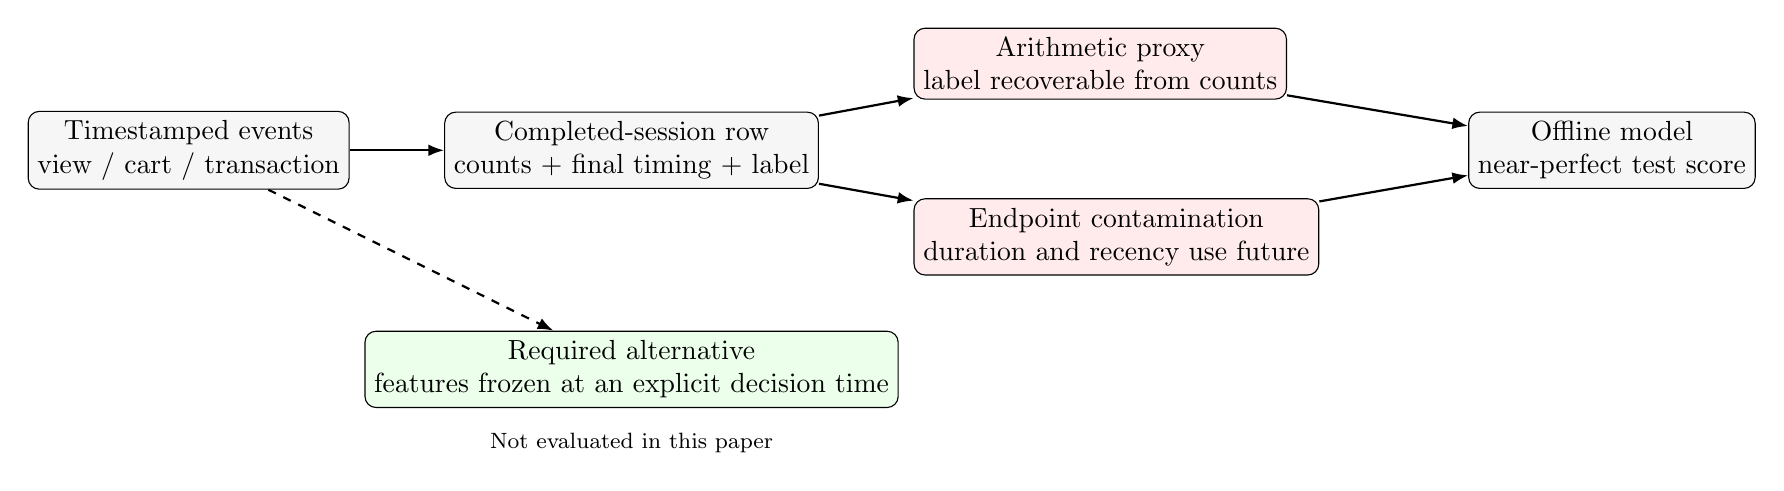
\begin{tikzpicture}[
  node distance=8mm and 12mm,
  box/.style={draw,rounded corners,align=center,minimum height=9mm,minimum width=31mm,fill=gray!7},
  bad/.style={draw,rounded corners,align=center,minimum height=9mm,minimum width=36mm,fill=red!8},
  good/.style={draw,rounded corners,align=center,minimum height=9mm,minimum width=36mm,fill=green!8},
  arr/.style={-{Latex[length=2mm]},thick}
]
\node[box] (events) {Timestamped events\\view / cart / transaction};
\node[box,right=of events] (complete) {Completed-session row\\counts + final timing + label};
\node[bad,right=of complete,yshift=11mm] (proxy) {Arithmetic proxy\\label recoverable from counts};
\node[bad,right=of complete,yshift=-11mm] (endpoint) {Endpoint contamination\\duration and recency use future};
\node[box,right=23mm of proxy,yshift=-11mm] (offline) {Offline model\\near-perfect test score};
\draw[arr] (events)--(complete);
\draw[arr] (complete)--(proxy);
\draw[arr] (complete)--(endpoint);
\draw[arr] (proxy)--(offline);
\draw[arr] (endpoint)--(offline);
\node[good,below=18mm of complete] (boundary) {Required alternative\\features frozen at an explicit decision time};
\draw[arr,dashed] (events)--(boundary);
\node[align=center,below=2mm of boundary,font=\footnotesize] {Not evaluated in this paper};
\end{tikzpicture}%
}
\caption{How completed-session construction changes the prediction problem. The upper path is audited here; the lower path represents the point-in-time design required for future online evaluation.}
\label{fig:concept}
\end{figure*}

This distinction prevents a common category error. Offline evaluation is not automatically invalid: historical events can be truncated to emulate a real decision boundary. Conversely, streaming infrastructure does not guarantee validity if each emitted record already contains future-dependent aggregates.

\subsection{Feature-Lineage Audit Procedure}
The preprocessing notebook, original model notebook, corrected training scripts, and derived session table were inspected. Each feature was traced to the event types and timestamps from which it was constructed. The audit proceeded in five steps: the label event and prediction boundary were defined; direct and algebraically reconstructable target fields were identified; durations and recencies were checked for use of the final session event; preprocessing parameters were checked for training-only estimation; and models were retrained under controlled feature ablations.

This order is important. Removing the explicit transaction-count column is insufficient if the same quantity can be reconstructed from other columns. Likewise, removing transaction count does not repair a duration whose endpoint is the transaction timestamp.

\subsection{Feature Configurations and Evaluation Protocol}
Four feature configurations were constructed from the supplied cart-session table. The \emph{target-proxy} condition contains total event, view, and add-to-cart counts, deliberately retaining the deterministic identity as a positive control. The \emph{original completed-session} condition contains the seven features used in the cart-session benchmark: view count, add-to-cart count, view-to-cart ratio, unique items, final session age, mean inter-event interval, and final cart recency. The \emph{timing-only} condition contains the three endpoint-dependent temporal variables. The \emph{counts-only} condition contains view count, add-to-cart count, view-to-cart ratio, and unique items.

The counts-only condition is not claimed to be online valid because the counts still summarize completed histories. It is a conservative diagnostic ablation that removes the two specifically identified channels: the exact count identity and completed-endpoint timing. Table~\ref{tab:audit} records the validity judgment for each feature group.

\begin{table}[t]
\caption{Feature validity relative to a pre-outcome scoring boundary.}
\label{tab:audit}
\centering
\scriptsize
\begin{tabularx}{\columnwidth}{@{}L{0.27\columnwidth}L{0.22\columnwidth}Y@{}}
\toprule
Feature/group & Audit result & Reason \\
\midrule
Transaction count & Invalid & Directly defines the label. \\
Total + view + cart counts & Invalid jointly & Transaction count is recovered exactly by subtraction. \\
Final session age & Invalid & Uses the completed endpoint and includes transaction timing for positive sessions. \\
Mean interval over full session & Invalid & Includes intervals to later events and potentially the transaction. \\
Recency to final event & Invalid & The reference endpoint is unknown during an active session. \\
Completed view/cart/item counts & Hindsight-dependent & No exact label identity, but actions after a possible decision time are included. \\
Training-only scaling/clipping & Valid preprocessing & Parameters are estimated without test-partition information. \\
\bottomrule
\end{tabularx}
\end{table}

Logistic regression and XGBoost \cite{chen2016} were evaluated across five stratified 80/20 holdouts with seeds 11, 22, 33, 42, and 55. A decision tree and random forest \cite{breiman2001} were additionally evaluated with seed 42 to reproduce the broader comparison in the original artifact. Class weighting was used for logistic regression and the tree models; XGBoost used the negative-to-positive class ratio as \texttt{scale\_pos\_weight}. Continuous features were capped at their 99th percentile using thresholds estimated from the training partition. Logistic regression was standardized through a training-only pipeline implemented with scikit-learn \cite{pedregosa2011}.

ROC-AUC was used to assess ranking performance. PR-AUC was also reported because positive-class prevalence was 27.17\%. Accuracy, precision, recall, and F1 were reported for the seed-42 reproduction at a threshold of 0.5. Standard deviations across holdouts are descriptive stability measures, not confidence intervals from independent samples.

\section{Leakage Mechanisms}
The evidence emerged in stages. The initial all-session score triggered the audit; the cart-session benchmark removed the explicit arithmetic identity but retained endpoint-dependent timing; and the controlled reanalysis separated these mechanisms under a common protocol. Table~\ref{tab:chronology} distinguishes historical triggers from primary evidence.

\begin{table*}[t]
\caption{Development chronology and evidential role.}
\label{tab:chronology}
\centering
\small
\setlength{\tabcolsep}{4pt}
\begin{tabularx}{\textwidth}{@{}L{0.15\textwidth}L{0.20\textwidth}L{0.10\textwidth}YL{0.10\textwidth}@{}}
\toprule
Stage & Population and model & ROC-AUC & What the stage revealed & Role \\
\midrule
Initial signal validation & 1,761,640 sessions; logistic regression, five-fold cross-validation & 0.9969 & Total count and component counts recover transaction count; scaling was fitted before cross-validation. & Audit trigger \\
Cart-session benchmark & 43,917 cart sessions; XGBoost & 0.9946 & Removing total count did not remove completed-endpoint timing contamination. & Historical benchmark \\
Reported non-transaction timing & Logistic regression, XGBoost, and hybrid LSTM & 0.654--0.686 & Transaction events were excluded from timing, but features still used the completed non-transaction history. & Supporting context \\
Controlled audit & Same cart-session table; four feature configurations; repeated holdouts & 0.606--1.000 & Separates the deterministic count proxy, endpoint timing, and residual completed-session counts under one protocol. & Primary evidence \\
\bottomrule
\end{tabularx}
\end{table*}

The main project report records ROC-AUC values of 0.6540 for logistic regression, 0.6860 for XGBoost, and 0.6654 for a hybrid LSTM after temporal variables were recomputed without transaction events. These results are useful corroborating evidence: the near-perfect performance disappears, and the more complex sequential model does not outperform the corrected tree baseline. They are not merged into the controlled ablation because they still summarize each complete non-transaction history: excluding transaction events moves the endpoint, but it does not remove the dependence on an endpoint that becomes known only after the session has closed. The training scripts for that path are retained, but the reported values predate the present protocol and were not regenerated under its repeated-holdout design with training-only preprocessing. The workshop-stage version of this study therefore treats them as development context rather than primary evidence.

\subsection{Arithmetic Target Reconstruction}
\label{sec:proxy}
The event vocabulary contains only three categories, while the session table stores total events, views, add-to-cart actions, and transaction count. Consequently,
\begin{equation}
\begin{aligned}
\texttt{transaction\_count}={}&\texttt{event\_count}-\texttt{view\_count}\\
&-\texttt{addtocart\_count}.
\end{aligned}
\label{eq:proxy}
\end{equation}
Equation~\ref{eq:proxy} holds for all 43,917 rows in the supplied table. The binary label also satisfies
\begin{equation}
 y_s=\mathbb{1}[\texttt{transaction\_count}_s>0]
\label{eq:label}
\end{equation}
for every row. The label therefore remains deterministically available after the explicit transaction column is removed, provided that the three component counts remain. This is an illegitimate-feature leakage mechanism in the sense of Kaufman et al. \cite{kaufman2012}. It explains why a linear classifier achieved an apparently exceptional score in the initial validation.

\subsection{Completed-Endpoint Timing Contamination}
\label{sec:endpoint}
The later cart-session benchmark excluded \texttt{event\_count} and therefore removed the exact identity. It nevertheless retained final session age, mean inter-event interval over the complete sequence, and recency from the last cart action to the final event. For purchased sessions, these calculations include the transaction event. For abandoned sessions, the endpoint is the final observed event before inactivity closes the session. The endpoint is therefore post-decision and selected differently by outcome.

Figure~\ref{fig:timing} shows the class-conditional medians. Purchased sessions have a median completed-session age of 821.03 seconds, compared with 172.44 seconds for abandoned sessions. Median recency from the last cart action is 330.82 seconds for purchased sessions and zero for abandoned sessions. Moreover, 60.6\% of abandoned sessions have zero cart recency because their final event is an add-to-cart action, compared with 2.1\% of purchased sessions.

\begin{figure}[t]
\centering
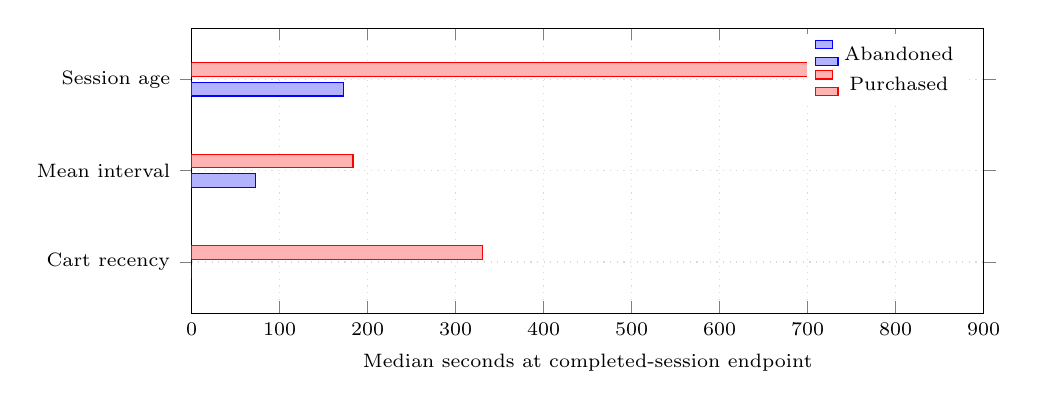
\begin{tikzpicture}
\begin{axis}[
  xbar,
  width=0.96\columnwidth,
  height=5.2cm,
  xmin=0,
  xmax=900,
  xlabel={Median seconds at completed-session endpoint},
  symbolic y coords={Cart recency,Mean interval,Session age},
  ytick=data,
  bar width=5pt,
  enlarge y limits=0.28,
  legend style={font=\scriptsize,at={(0.98,0.98)},anchor=north east,draw=none},
  tick label style={font=\scriptsize},
  label style={font=\scriptsize},
  grid=major,
  grid style={dotted,gray!30}
]
\addplot coordinates {(0,Cart recency) (72.77,Mean interval) (172.44,Session age)};
\addplot coordinates {(330.82,Cart recency) (183.29,Mean interval) (821.03,Session age)};
\legend{Abandoned,Purchased}
\end{axis}
\end{tikzpicture}
\caption{Class-conditional medians of endpoint-dependent timing features. The differences may contain genuine behavior, but the completed endpoint is unavailable at a pre-outcome decision time.}
\label{fig:timing}
\end{figure}

The distributional differences do not prove that every unit of predictive performance is caused by leakage. They show that a model can exploit information generated after the intended intervention point. A feature can be behaviorally meaningful and still be invalid for the claimed use case.

\subsection{Label Ambiguity at a Decision Time}
The first two mechanisms concern features. A third defect is located in the target itself and is therefore not repaired by any feature ablation.

The session-level rule assigns $y_s = 1$ when session $s$ contains at least one transaction event. This is well defined for a completed session, but it does not describe the outcome of a specific cart decision. A visitor may purchase one item and, in the same session, add a second item to the cart and leave without buying it. The session-level rule records this as a purchase, although one cart action was in fact abandoned.

The audited artifact contains a directly measurable instance of the problem. Of the 43,917 cart sessions, 172 contain a transaction that occurs \emph{before} the first add-to-cart event of that session. Under the session-level rule these sessions are labeled purchased, even though no cart action had yet taken place when the purchase occurred. A further 1,573 sessions contain a transaction that occurs strictly between the first and last add-to-cart action of the same session. Together these 1,745 sessions, 4.0\% of the modeling population, record a purchase event that cannot describe the outcome of at least one cart action they contain.

A label consistent with an intervention-time task must be tied to the decision point rather than to the session:
\begin{equation}
y_{s,k} = \mathbb{1}[\exists\, e_{s,j} : \mathrm{type}(e_{s,j}) = \texttt{transaction} \;\wedge\; t_{s,j} > t_{s,k}],
\label{eq:cutlabel}
\end{equation}
where $t_{s,k}$ is the cutoff timestamp. The outcome then belongs to the pair (session, decision point), and a session that has already converted before $t_{s,k}$ leaves the risk set rather than contributing a positive example.

This defect is easy to overlook because it produces no implausible score. It does not inflate performance in the manner of Sections~\ref{sec:proxy} and~\ref{sec:endpoint}; it silently changes the question being answered. It is reported here because the same session table supports both formulations, and only one of them corresponds to a decision a retailer could act on.

\subsection{Preprocessing Leakage}
Two weaker implementation issues were also found. In the initial all-session notebook, standardization was fitted before cross-validation. In the original cart-session notebook, 99th-percentile clipping thresholds were estimated on the full dataset before the train/test split. Both choices expose test-distribution information to training, although their likely effect is smaller than that of the feature-level mechanisms. In the controlled reanalysis, clipping thresholds and scaling parameters were learned separately within each training partition.

\section{Results}
The controlled results answer two questions: whether the original near-perfect pattern can be reproduced under isolated preprocessing, and how that pattern changes across the audited feature groups. Exact repeated-holdout values are reported alongside visual summaries.

\subsection{Reproduction of the Original Benchmark}
Using the original completed-session feature set and seed 42, the reanalysis reproduces the historical pattern closely. XGBoost reaches ROC-AUC 0.9948 and PR-AUC 0.9876; random forest reaches ROC-AUC 0.9837; decision tree reaches 0.9340; and logistic regression reaches 0.8249. The historical XGBoost value was 0.9946. The small difference is consistent with training-only clipping and software-version variation. Table~\ref{tab:original} shows that, when interpreted without a feature audit, the task appears exceptionally easy and nonlinear tree ensembles appear decisively superior.
\begin{table}[t]
\caption{Seed-42 results with the original completed-session feature set.}
\label{tab:original}
\centering
\scriptsize
\begin{tabular}{lrrrrrr}
\toprule
Model & Acc. & Prec. & Recall & F1 & ROC-AUC & PR-AUC \\
\midrule
Logistic regression & .777 & .591 & .580 & .585 & .825 & .599 \\
Decision tree & .841 & .642 & .941 & .763 & .934 & .834 \\
Random forest & .941 & .908 & .871 & .889 & .984 & .962 \\
XGBoost & .964 & .912 & .963 & .936 & .995 & .988 \\
\bottomrule
\end{tabular}
\end{table}

\subsection{Ablation Across Leakage Pathways}
Figure~\ref{fig:auc} reports mean ROC-AUC across the five holdouts. The target proxy yields 0.9944$\pm$0.0004 for logistic regression and 0.9997$\pm$0.0001 for XGBoost. The original completed-session feature set retains an XGBoost score of 0.9947$\pm$0.0005 after the exact count identity is removed. Timing features alone still yield 0.8688$\pm$0.0035. Once the three endpoint-dependent timing variables are removed, XGBoost falls to 0.6065$\pm$0.0024, while logistic regression reaches 0.6061$\pm$0.0035.

\begin{figure}[t]
\centering
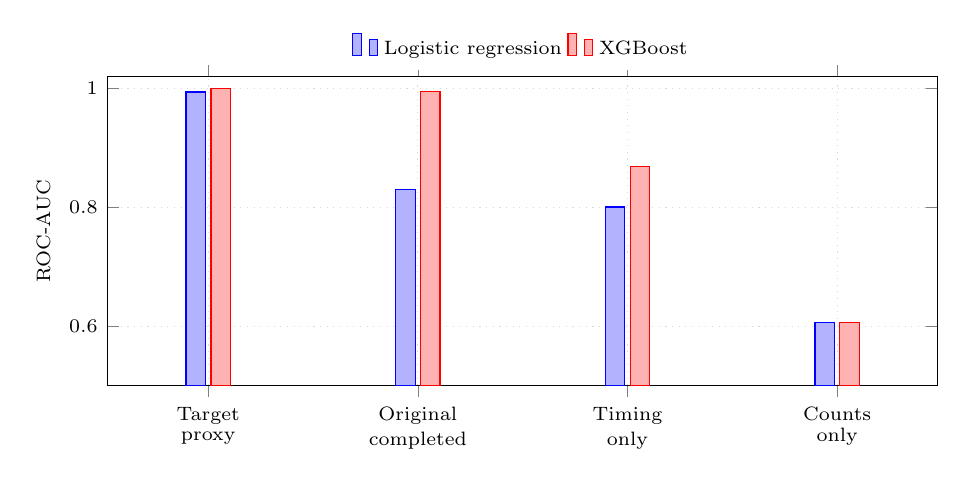
\begin{tikzpicture}
\begin{axis}[
  ybar,
  width=\columnwidth,
  height=5.5cm,
  ymin=0.5,
  ymax=1.02,
  ylabel={ROC-AUC},
  symbolic x coords={Proxy,Original,Timing,Counts},
  xtick=data,
  xticklabels={\shortstack{Target\\proxy},\shortstack{Original\\completed},\shortstack{Timing\\only},\shortstack{Counts\\only}},
  x tick label style={font=\scriptsize,align=center},
  tick label style={font=\scriptsize},
  label style={font=\scriptsize},
  bar width=7pt,
  enlarge x limits=0.16,
  legend style={font=\scriptsize,at={(0.5,1.02)},anchor=south,legend columns=2,draw=none},
  grid=major,
  grid style={dotted,gray!30}
]
\addplot coordinates {(Proxy,0.9944) (Original,0.8306) (Timing,0.8006) (Counts,0.6061)};
\addplot coordinates {(Proxy,0.9997) (Original,0.9947) (Timing,0.8688) (Counts,0.6065)};
\legend{Logistic regression,XGBoost}
\end{axis}
\end{tikzpicture}
\caption{Mean ROC-AUC across five repeated stratified holdouts. Counts-only remains a completed-session diagnostic, not an online evaluation.}
\label{fig:auc}
\end{figure}

Figure~\ref{fig:prauc} shows the same inflation pattern for precision-recall performance. XGBoost falls from 0.9992$\pm$0.0002 with the deterministic proxy to 0.9872$\pm$0.0010 with the original completed-session set, 0.6530$\pm$0.0106 with timing alone, and 0.3943$\pm$0.0032 with counts alone. Positive-class prevalence is 0.2717, so the final condition retains modest signal but nothing resembling the near-perfect benchmark. Table~\ref{tab:ablation} provides the exact means and standard deviations used in Figures~\ref{fig:auc} and~\ref{fig:prauc}.

\begin{figure}[t]
\centering
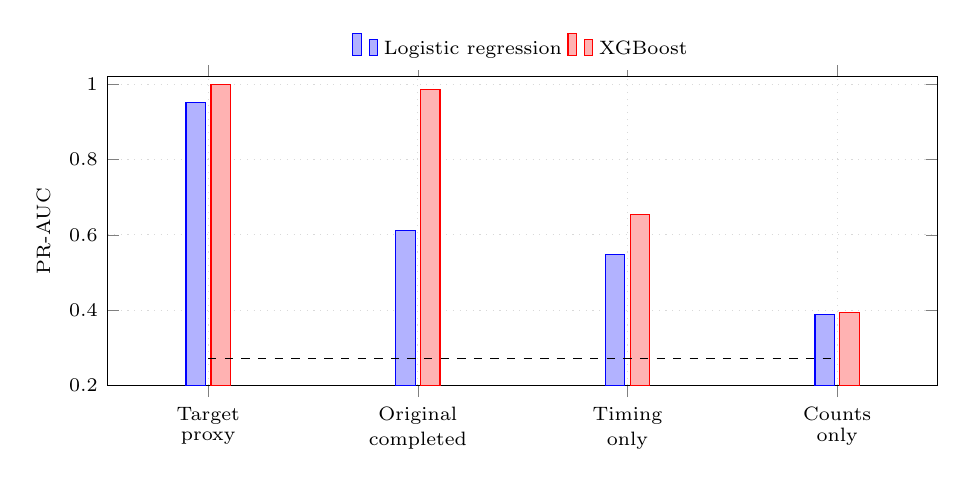
\begin{tikzpicture}
\begin{axis}[
  ybar,
  width=\columnwidth,
  height=5.5cm,
  ymin=0.2,
  ymax=1.02,
  ylabel={PR-AUC},
  symbolic x coords={Proxy,Original,Timing,Counts},
  xtick=data,
  xticklabels={\shortstack{Target\\proxy},\shortstack{Original\\completed},\shortstack{Timing\\only},\shortstack{Counts\\only}},
  x tick label style={font=\scriptsize,align=center},
  tick label style={font=\scriptsize},
  label style={font=\scriptsize},
  bar width=7pt,
  enlarge x limits=0.16,
  legend style={font=\scriptsize,at={(0.5,1.02)},anchor=south,legend columns=2,draw=none},
  grid=major,
  grid style={dotted,gray!30}
]
\addplot coordinates {(Proxy,0.9525) (Original,0.6123) (Timing,0.5476) (Counts,0.3895)};
\addplot coordinates {(Proxy,0.9992) (Original,0.9872) (Timing,0.6530) (Counts,0.3943)};
\addplot[black,dashed,sharp plot,forget plot] coordinates {(Proxy,0.2717) (Counts,0.2717)};
\legend{Logistic regression,XGBoost}
\end{axis}
\end{tikzpicture}
\caption{Mean PR-AUC across five repeated stratified holdouts. The dashed line marks positive-class prevalence.}
\label{fig:prauc}
\end{figure}

\begin{table}[t]
\caption{Repeated-holdout ablation (mean $\pm$ standard deviation).}
\label{tab:ablation}
\centering
\scriptsize
\begin{tabular}{llcc}
\toprule
Feature configuration & Model & ROC-AUC & PR-AUC \\
\midrule
\multirow{2}{*}{Target proxy}
 & Logistic regression & $.9944\pm.0004$ & $.9525\pm.0042$ \\
 & XGBoost & $.9997\pm.0001$ & $.9992\pm.0002$ \\
\midrule
\multirow{2}{*}{Original completed}
 & Logistic regression & $.8306\pm.0036$ & $.6123\pm.0082$ \\
 & XGBoost & $.9947\pm.0005$ & $.9872\pm.0010$ \\
\midrule
\multirow{2}{*}{Timing only}
 & Logistic regression & $.8006\pm.0032$ & $.5476\pm.0094$ \\
 & XGBoost & $.8688\pm.0035$ & $.6530\pm.0106$ \\
\midrule
\multirow{2}{*}{Counts only}
 & Logistic regression & $.6061\pm.0035$ & $.3895\pm.0049$ \\
 & XGBoost & $.6065\pm.0024$ & $.3943\pm.0032$ \\
\bottomrule
\end{tabular}
\end{table}

\subsection{Interpretation of Model Complexity}
Under the original feature set, XGBoost appears vastly superior to logistic regression. Under counts only, their mean ROC-AUC values differ by 0.0004. This convergence does not imply that model choice is generally irrelevant. It shows that the apparent algorithmic advantage in this experiment was conditional on features that violated the intended information boundary.

The ablation should not be interpreted as a precise causal decomposition. Removing a feature block changes the fitted function and can remove legitimate behavioral signal together with invalid information. The defensible conclusion is structural: the near-perfect result does not survive when variables tied to the completed endpoint are unavailable. Feature validity therefore had to be established before model rankings could be interpreted.

\section{Discussion}
The audit changes the scientific meaning of the original project. What first appeared to be a high-performing prediction system is better understood as evidence that the data representation answered a different, retrospective question.

\subsection{What Completed Sessions Actually Predict}
The first failure mode is deterministic. Removing the obvious label column does not prevent leakage when the same label-generating count can be recovered algebraically from other inputs. Feature importance is a weak defense because a nonlinear model can distribute the identity across several columns. The relevant test is arithmetic closure: whether the target or a target-defining event count can be reconstructed from the remaining feature set.

The second failure mode is temporal. Final duration and recency variables can be commercially meaningful, yet they describe what the complete session looked like after its outcome was known. A pre-outcome model asks what was observable at a specified event or clock time. Completed-session construction silently shifts the observation boundary to the endpoint and makes that endpoint outcome-dependent.

There is no universal ROC-AUC threshold above which leakage must exist. Nevertheless, an implausibly strong score for a noisy behavioral outcome should trigger a feature-lineage audit rather than immediate optimization. A high offline score is not by itself proof of leakage: Esmeli and Gokce report ROC-AUC of 0.990 on a comparable post-add-to-cart task with a reported feature set containing neither an arithmetically closed count group nor endpoint-anchored timing variables \cite{esmeli2025}. The claim advanced here is correspondingly narrower. In the audited artifact the specific mechanisms were located, and the score did not survive their removal. The strongest scientific result is therefore not the near-perfect score; it is the demonstration that the score did not measure the intended intervention-time task.

\subsection{Practical Leakage-Audit Checklist}
Before a session-level prediction result is accepted, nine questions should be answered:
\begin{enumerate}
    \item What exact event or time defines the prediction moment?
    \item Which event creates the label?
    \item Does the label describe the outcome of the specific decision, or only of the session that contains it?
    \item Can that event count be reconstructed from other counts?
    \item Does any duration, recency, or average use the final session event?
    \item Is the endpoint selected differently for positive and negative cases?
    \item Are clipping, scaling, feature selection, and imputation fitted using training data only?
    \item Does performance remain plausible after suspicious feature groups are removed?
    \item Can the experiment be rerun from code and preserved outputs?
\end{enumerate}
The checklist is intentionally simple. None of the nine questions requires additional computation; each can be answered from the data dictionary, the preparation code, and the definition of the intended intervention. Leakage often survives because attention is directed toward architecture and hyperparameters while the semantics of a few columns remain unexamined.

\subsection{Implications for E-Commerce Experiments}
The intended business action should be specified before data are aggregated. A discount displayed immediately after the first cart action, a reminder issued after two minutes of inactivity, and a follow-up email sent after session expiration are three different prediction tasks. Each permits a different feature set and requires a different outcome horizon. Treating them all as ``cart-abandonment prediction'' obscures these boundaries.

A genuine in-session study should assign every training example an explicit cutoff timestamp, an observation window ending at that cutoff, and an outcome window beginning afterward. Features should be regenerated from each observed prefix, and labels should be assigned according to Equation~\ref{eq:cutlabel} rather than at the session level. This design is more expensive than storing one row per completed session, but it prevents the target event from participating in its own prediction and allows performance to be studied as a function of decision time.

\subsection{Threats to Validity}
This study audits one public dataset and one sessionization scheme. The absolute estimates may differ for another retailer, event taxonomy, or inactivity boundary. The five random holdouts share observations, and some visitors contribute multiple sessions. A visitor-grouped or temporal split could therefore change generalization estimates, although it would not alter the deterministic identity in Equations~\ref{eq:proxy} and~\ref{eq:label}.

The counts-only condition is not a leakage-free production benchmark because its counts are computed after the complete session. Likewise, timing-only discrimination may combine genuine behavior with invalid future information, so the experiment cannot assign every unit of AUC causally to leakage. The main project report describes a later recomputation that excludes transaction events, but it also remains a completed-history evaluation. Those scores were produced before the present protocol was defined and were not regenerated under its five-seed, training-only preprocessing design, so they are not directly comparable with the ablation reported here. Consequently, the 0.654--0.686 results are treated as supporting context, and no corrected online-valid score is claimed. Finally, no live deployment or intervention experiment was performed.

\section{Reproducibility Statement}
The primary audit has been re-executed from the 43,917-row derived cart-session table and a standalone reanalysis script. A submission package should include that table, the exact five seed values, generated metric files, figure inputs, and an environment specification. Before model fitting, the script should assert the count identity in Equation~\ref{eq:proxy} and the target identity in Equation~\ref{eq:label}. Clipping and scaling parameters must then be learned from each training partition only.

The event-level preparation path has since been re-executed from the raw file. Re-running the original cleaning rules on the 2,756,101 raw events reproduces the reported figures exactly: 35 suspected automated visitors and 491 events removed, leaving 2,755,610 events, with a row-for-row match against the retained cleaned artifact on visitor identifier, timestamp, event type, and item identifier. The removed events comprise 431 views and 60 add-to-cart actions and no transactions, indicating that the heuristic filter discarded no converting visitor. The controlled comparisons were independently re-executed under the protocol of Table~\ref{tab:settings} using scikit-learn 1.8.0, XGBoost 3.3.0, NumPy 2.3.3, and pandas 2.3.2. Nineteen of the twenty reported cells in Tables~\ref{tab:original} and~\ref{tab:ablation} reproduced within $\pm 0.0007$. The exception is the timing-only XGBoost PR-AUC, which returned 0.6563 against the reported 0.6530; this is the cell with the largest reported standard deviation ($\pm 0.0106$), and the difference lies within one standard error of the reported mean. The published values are retained, and the re-execution values are recorded in the accompanying provenance table rather than substituted for them.

A provenance table mapping each published figure to the script that produces it is distributed with the submission package. One figure in the underlying project report, the log of intermediate LSTM development iterations, is recorded there as untraced: no sweep code for those configurations was preserved, and no value from that table is used as evidence in this paper. Table~\ref{tab:settings} summarizes the settings required to rerun the controlled comparisons. The objective is not to optimize a state-of-the-art classifier, but to test whether the interpretation changes when invalid feature groups are removed.

\begin{table}[t]
\caption{Model and preprocessing settings in the audit.}
\label{tab:settings}
\centering
\scriptsize
\begin{tabularx}{\columnwidth}{@{}L{0.30\columnwidth}Y@{}}
\toprule
Component & Setting \\
\midrule
Data split & Stratified 80/20; seeds 11, 22, 33, 42, 55 \\
Outlier handling & Upper 99th-percentile cap fitted on each training partition \\
Logistic regression & Balanced class weights; 2,000 maximum iterations; training-only standardization \\
Decision tree & Balanced class weights; maximum depth 8; seed-42 reproduction \\
Random forest & 100 trees; balanced class weights; seed-42 reproduction \\
XGBoost & 100 trees; class-ratio weight; histogram tree method \\
Primary metrics & ROC-AUC and PR-AUC \\
Secondary metrics & Accuracy, precision, recall, and F1 at threshold 0.5 \\
\bottomrule
\end{tabularx}
\end{table}

The deterministic identities, class-conditional summaries, seed-42 four-model benchmark, and five-holdout logistic regression and XGBoost ablation are reproducible when the described aggregate table and audit script are supplied. The cleaned event stream and the training scripts used for the later non-transaction timing experiment are also retained, but those scores were generated under an earlier single-split protocol and were not regenerated for this paper. The paper therefore excludes them from its primary tables and restricts its central claims to results obtained under one common rerun protocol.

\section{Conclusion}
Completed-session tables can make cart-abandonment prediction appear much easier than the intended intervention-time task. In the audited artifact, one group of counts reconstructed the transaction label exactly, while completed-endpoint timing preserved near-perfect XGBoost performance after that identity was removed. Across the diagnostic configurations, mean XGBoost ROC-AUC was 0.9997 with the deterministic proxy, 0.9947 with the original completed-session features, and 0.6065 after endpoint-dependent timing was removed. Logistic regression converged to essentially the same final level.

The conclusion is methodological rather than algorithmic: an offline score is not interpretable until every feature is mapped to the stated decision time. The next research step is to generate explicit pre-outcome prefixes and evaluate temporal and visitor-grouped generalization. The present study establishes the prerequisite for that work: the model must be tested only on information that could have been observed when a real intervention was still possible.

\section*{Acknowledgment}
The authors thank Bah\c{c}e\c{s}ehir University's Department of Artificial Intelligence Engineering for the computational resources and course environment (Big Data and Analytics) that supported this study.

\section*{Declarations}
\textit{Conflict of Interest:} The authors declare no conflict of interest.

\textit{Funding:} This research received no external funding.

\textit{Declaration on Generative AI:} This project was developed with the assistance of generative AI systems (Claude, Anthropic; ChatGPT, OpenAI) over a period of approximately seven months. Their use included iterative assistance with analysis code, exploratory discussion of candidate interpretations of observed patterns, and drafting and formatting support for the manuscript, including its conversion to the journal's template. Throughout the project, the authors directed the research questions and overall audit design, executed and validated all code against the underlying data, and critically evaluated, tested, and verified every interpretive claim before its inclusion in the manuscript (see the Reproducibility Statement for details on the independent re-verification of the quantitative results). The authors assume full responsibility for the accuracy, originality, and scientific validity of the manuscript. No generative AI system is listed as an author.

\bibliographystyle{IEEEtran}
\bibliography{references_revised}

\end{document}
